% --------------------------------------
% Document Class
% --------------------------------------
\documentclass[a4paper,11pt]{article}
% --------------------------------------



% --------------------------------------
% Use Package
% --------------------------------------

\usepackage[francais]{babel}
\usepackage{ucs}
\usepackage[utf8]{inputenc}
\usepackage[T1]{fontenc}

\usepackage{makeidx}
\usepackage{color}
\usepackage{graphicx}
\usepackage{float}
\usepackage[hidelinks]{hyperref} 
\usepackage{geometry}
%\usepackage{lastpage}
%\usepackage{marginnote}
\usepackage{fancyhdr}
%\usepackage{titlesec}
%\usepackage{framed}
\usepackage{amsmath}
\usepackage{empheq}
\usepackage{array}
\usepackage{multicol}
\usepackage{csquotes}
%\usepackage{adjustbox}

% insert code
\usepackage{listings}

% define our color
\usepackage{xcolor}

% code color
\definecolor{ligthyellow}{RGB}{250,247,220}
\definecolor{darkblue}{RGB}{5,10,85}
\definecolor{ligthblue}{RGB}{1,147,128}
\definecolor{darkgreen}{RGB}{8,120,51}
\definecolor{darkred}{RGB}{160,0,0}

% other color
\definecolor{ivi}{RGB}{141,107,185}

\def\verticaltext#1{\rotatebox[origin=c]{90}{\x{#1}}}


\lstset{
    language=python,
    captionpos=b,
    extendedchars=true,
    frame=lines,
    numbers=left,
    numberstyle=\tiny,
    numbersep=5pt,
    keepspaces=true,
    breaklines=true,
    showspaces=false,
    showstringspaces=false,
    breakatwhitespace=false,
    stepnumber=1,
    showtabs=false,
    tabsize=3,
    basicstyle=\small\ttfamily,
    backgroundcolor=\color{ligthyellow},
    keywordstyle=\color{ligthblue},
    morekeywords={include, printf, uchar},
    identifierstyle=\color{darkblue},
    commentstyle=\color{darkgreen},
    stringstyle=\color{darkred},
}


% --------------------------------------



% --------------------------------------
% Page setting
% --------------------------------------
%\pagestyle{empty}
\setlength{\headheight}{15pt}

\setcounter{secnumdepth}{3}
\setcounter{tocdepth}{2}

\makeatletter
\@addtoreset{chapter}{part}
\makeatother 

\hypersetup{       % parametrage des hyperliens
  colorlinks=true,  % colorise les liens
  breaklinks=true,  % permet les retours à la ligne pour les liens 
                    % trop longs
  urlcolor= blue,   % couleur des hyperliens
  linkcolor= black, % couleur des liens internes aux documents 
                    % (index, figures, tableaux, equations,...)
  citecolor= green  % couleur des liens vers les references 
                    % bibliographiques
}

% --------------------------------------

% --------------------------------------
% Information
% --------------------------------------
\title{
  \noindent\hrulefill \\
  \vspace{10mm}
  \textbf{Compte-rendu VisA} \\
  \vspace{5mm}
  TP: Approche de la logique floue.
}

\author{Gaëtan DEFLANDRE}
% --------------------------------------

\definecolor{myColor}{rgb}{0.5, 0.1, 0.75}

% --------------------------------------
% Begin content
% --------------------------------------
\begin{document}

\maketitle
\noindent\hrulefill \\


\section*{Introduction}

Dans ces TPs, nous poursuivons l'étude de la logique floue. Nous allons 
utiliser les principes de cette logique pour segmenter des images. \\

Durant ces TPs, nous implémentons en logique floue des algorithmes 
classifications de classes dans les images. En logique booléenne, 
certaines de ces méthodes sont très utilisés, telles que le C-Means. Il 
existe la variante floue de cette méthode, elle s'apelle FCM (Fuzzy 
C-Means). Ainsi, nous verrons différents algorithmes de classification 
floue.\\


\newpage



Lors de ces TPs, nous utilisons pour image de référence, une image 
contenant six classes. Cette image est la suivante:

\begin{figure}[H]
  \begin{center} 
    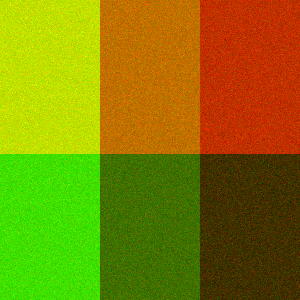
\includegraphics[width=180px]{../img/6_classes_RGB.png}
    \caption{\texttt{6\_classes\_RGB.tif} utilisé pour la classification.}
  \end{center}
\end{figure}

\section{Algorithme Fuzzy C-Means}

\subsection{Résultats}

\begin{table}[H]
  \begin{center}
    \begin{tabular}{|l|c|}
      \hline
      Nombre de classes & 6 \\
      \hline
      Valeur de m & 2 \\
      \hline
      Nombre d'itération & 100 \\
      \hline
      \shortstack{ Valeur de seuil \\ de stabilité } & 0.000001 \\
      \hline
      Randomisation & 1 \\
      \hline
    \end{tabular}
    \caption{Tableau des paramétres utiliser pour l'algorithme de FCM}
  \end{center}
\end{table}


\begin{figure}[H]
  \begin{center} 
    
\includegraphics[width=180px]{../img/segFCM.png}
    \caption{Image résultante avec l'algorithme FCM}
  \end{center}
\end{figure}

\section{Algorithme Hard C-Means}

\subsection{Résultats}

\begin{table}[H]
  \begin{center}
    \begin{tabular}{|l|c|}
      \hline
      Nombre de classes & 6 \\
      \hline
      Valeur de m & 1 \\
      \hline
      Nombre d'itération & 1000 \\
      \hline
      \shortstack{ Valeur de seuil \\ de stabilité }  & 0.000001 \\
      \hline
      Randomisation & 1 \\
      \hline
    \end{tabular}
    \caption{Tableau des paramétres utiliser pour l'algorithme de HCM}
  \end{center}
\end{table}


\begin{figure}[H]
  \begin{center} 
    
\includegraphics[width=180px]{../img/segHCM.png}
    \caption{Image résultante avec l'algorithme HCM}
  \end{center}
\end{figure}

\section{Algorithme Possibilistic C-Means}

\begin{table}[H]
  \begin{center}
    \begin{tabular}{|l|c|}
      \hline
      Nombre de classes & 6 \\
      \hline
      Valeur de m & 1 \\
      \hline
      Nombre d'itération & 1000 \\
      \hline
      \shortstack{ Valeur de seuil \\ de stabilité }  & 0.000001 \\
      \hline
      Randomisation & 1 \\
      \hline
    \end{tabular}
    \caption{Tableau des paramétres utiliser pour l'algorithme de PCM}
  \end{center}
\end{table}


\begin{figure}[H]
  \begin{center} 
    
\includegraphics[width=180px]{../img/segHCM.png}
    \caption{Image résultante avec l'algorithme PCM}
  \end{center}
\end{figure}

\section{Algorithme de Davé}

\subsection{Résultats}

\begin{table}[H]
  \begin{center}
    \begin{tabular}{|l|c|}
      \hline
      Nombre de classes & 6 \\
      \hline
      Valeur de m & 2 \\
      \hline
      Nombre d'itération & 5000 \\
      \hline
      \shortstack{ Valeur de seuil \\ de stabilité }  & 0.0000001 \\
      \hline
      Randomisation & 1 \\
      \hline
    \end{tabular}
    \caption{Tableau des paramétres utiliser pour l'algorithme de Davé}
  \end{center}
\end{table}


\begin{figure}[H]
  \begin{center} 
    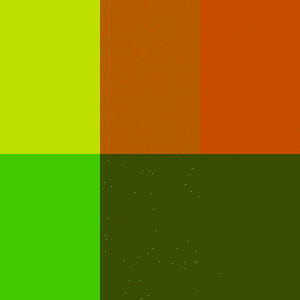
\includegraphics[width=180px]{../img/segDave.png}
    \caption{Image résultante avec l'algorithme de Davé}
  \end{center}
\end{figure}

\section*{Conclusion}

Nous pouvons conclure que les différentes méthodes vues lors de ces TPs, ne sont 
pas véritablement des algorithmes de segmentations. En effet, elles calculent 
des degrés d'appartenance qui ne permettent pas de segmenter directement les 
images.\\

Pour segmenter les images dont les degrés d'appartenance aux classes ont été calculés,
il faut définir des heuristiques qui vont séparer les pixels.\\


\end{document}
